% Created 2023-03-17 fr 15:10
% Intended LaTeX compiler: pdflatex
\documentclass[12pt]{article}

%%%% settings when exporting code %%%% 

\usepackage{listings}
\lstdefinestyle{code-small}{
backgroundcolor=\color{white}, % background color for the code block
basicstyle=\ttfamily\small, % font used to display the code
commentstyle=\color[rgb]{0.5,0,0.5}, % color used to display comments in the code
keywordstyle=\color{black}, % color used to highlight certain words in the code
numberstyle=\ttfamily\tiny\color{gray}, % color used to display the line numbers
rulecolor=\color{black}, % color of the frame
stringstyle=\color[rgb]{0,.5,0},  % color used to display strings in the code
breakatwhitespace=false, % sets if automatic breaks should only happen at whitespace
breaklines=true, % sets automatic line breaking
columns=fullflexible,
frame=single, % adds a frame around the code (non,leftline,topline,bottomline,lines,single,shadowbox)
keepspaces=true, % % keeps spaces in text, useful for keeping indentation of code
literate={~}{$\sim$}{1}, % symbol properly display via latex
numbers=none, % where to put the line-numbers; possible values are (none, left, right)
numbersep=10pt, % how far the line-numbers are from the code
showspaces=false,
showstringspaces=false,
stepnumber=1, % the step between two line-numbers. If it's 1, each line will be numbered
tabsize=1,
xleftmargin=0cm,
emph={anova,apply,class,coef,colnames,colNames,colSums,dim,dcast,for,ggplot,head,if,ifelse,is.na,lapply,list.files,library,logLik,melt,plot,require,rowSums,sapply,setcolorder,setkey,str,summary,tapply},
aboveskip = \medskipamount, % define the space above displayed listings.
belowskip = \medskipamount, % define the space above displayed listings.
lineskip = 0pt} % specifies additional space between lines in listings
\lstset{style=code-small}
%%%% packages %%%%%

\usepackage[utf8]{inputenc}
\usepackage[T1]{fontenc}
\usepackage{lmodern}
\usepackage{textcomp}
\usepackage{color}
\usepackage{graphicx}
\usepackage{grffile}
\usepackage{wrapfig}
\usepackage{rotating}
\usepackage{longtable}
\usepackage{multirow}
\usepackage{multicol}
\usepackage{changes}
\usepackage{pdflscape}
\usepackage{geometry}
\usepackage[normalem]{ulem}
\usepackage{amssymb}
\usepackage{amsmath}
\usepackage{amsfonts}
\usepackage{dsfont}
\usepackage{array}
\usepackage{ifthen}
\usepackage{hyperref}
\usepackage{natbib}
%
%%%% specifications %%%%
%
\usepackage{ifthen}
\usepackage{xifthen}
\usepackage{xargs}
\usepackage{xspace}
\newcommand\Rlogo{\textbf{\textsf{R}}\xspace} %
\RequirePackage{fancyvrb}
\DefineVerbatimEnvironment{verbatim}{Verbatim}{fontsize=\small,formatcom = {\color[rgb]{0.5,0,0}}}
\RequirePackage{colortbl} % arrayrulecolor to mix colors
\RequirePackage{setspace} % to modify the space between lines - incompatible with footnote in beamer
\renewcommand{\baselinestretch}{1.1}
\geometry{top=1cm}
\RequirePackage{changepage}
\RequirePackage{colortbl} % arrayrulecolor to mix colors
\RequirePackage{pifont}
\RequirePackage{relsize}
\newcommand{\Cross}{{\raisebox{-0.5ex}%
{\relsize{1.5}\ding{56}}}\hspace{1pt} }
\newcommand{\Valid}{{\raisebox{-0.5ex}%
{\relsize{1.5}\ding{52}}}\hspace{1pt} }
\newcommand{\CrossR}{ \textcolor{red}{\Cross} }
\newcommand{\ValidV}{ \textcolor{green}{\Valid} }
\usepackage{stackengine}
\usepackage{scalerel}
\newcommand\Warning[1][3ex]{%
\renewcommand\stacktype{L}%
\scaleto{\stackon[1.3pt]{\color{red}$\triangle$}{\tiny\bfseries !}}{#1}%
\xspace
}
\hypersetup{
citecolor=[rgb]{0,0.5,0},
urlcolor=[rgb]{0,0,0.5},
linkcolor=[rgb]{0,0,0.5},
}
\RequirePackage{epstopdf} % to be able to convert .eps to .pdf image files
\RequirePackage{capt-of} %
\RequirePackage{caption} % newlines in graphics
\RequirePackage{enumitem} % to be able to convert .eps to .pdf image files
\definecolor{light}{rgb}{1, 1, 0.9}
\definecolor{lightred}{rgb}{1.0, 0.7, 0.7}
\definecolor{lightblue}{rgb}{0.0, 0.8, 0.8}
\newcommand{\darkblue}{blue!80!black}
\newcommand{\darkgreen}{green!50!black}
\newcommand{\darkred}{red!50!black}
\usepackage{mdframed}
\newcommand{\first}{1\textsuperscript{st} }
\newcommand{\second}{2\textsuperscript{nd} }
\newcommand{\third}{3\textsuperscript{rd} }
\date{\today}
\title{Results simulation study DelayedGSD}
\hypersetup{
 colorlinks=true,
 pdfauthor={},
 pdftitle={Results simulation study DelayedGSD},
 pdfkeywords={},
 pdfsubject={},
 pdfcreator={Emacs 27.2 (Org mode 9.5.2)},
 pdflang={English}
 }
\begin{document}

\maketitle

\section{Rejection rate}
\label{sec:orge7abcfb}

Power by method (columns) and scenario (rows): \hfill (nominal level 80\%)
\begin{verbatim}
 scenario     N missing binding  fixC ar method 1 method 2 method 3
        1 10000    TRUE    TRUE FALSE 10    81.00    80.79    80.45
        3 10000    TRUE    TRUE FALSE  5    80.60    80.45    80.21
        5 10000    TRUE    TRUE  TRUE 10    79.81    80.41    80.39
        7 10000    TRUE    TRUE  TRUE  5    80.00    80.46    80.08
        9 10000    TRUE   FALSE  TRUE 10    80.50    80.85    80.91
       11 10000    TRUE   FALSE  TRUE  5    80.73    80.82    80.75
       13 10000    TRUE   FALSE FALSE 10    80.67    80.60    80.65
       15 10000    TRUE   FALSE FALSE  5    80.65    80.64    80.46
       17 10000   FALSE    TRUE FALSE  5    80.31    80.28    79.93
\end{verbatim}
\Warning slightly too high power for some scenario

\bigskip

Type 1 error by method (columns) and scenario (rows): \hfill (nominal level 2.5\%)
\begin{verbatim}
 scenario     N missing binding  fixC ar method 1 method 2 method 3
        2 10000    TRUE    TRUE FALSE 10     2.46     2.53     2.40
        4 10000    TRUE    TRUE FALSE  5     2.42     2.41     2.40
        6 10000    TRUE    TRUE  TRUE 10     2.25     2.25     2.45
        8 10000    TRUE    TRUE  TRUE  5     2.42     2.39     2.50
       10 10000    TRUE   FALSE  TRUE 10     2.16     2.18     2.31
       12 10000    TRUE   FALSE  TRUE  5     2.36     2.35     2.38
       14 10000    TRUE   FALSE FALSE 10     2.44     2.44     2.58
       16 10000    TRUE   FALSE FALSE  5     2.51     2.50     2.58
       18 10000   FALSE    TRUE FALSE  5     2.46     2.44     2.45
\end{verbatim}
Type 1 error slightly below nominal level when fixC is TRUE (as expected?)

\clearpage

\begin{figure}[!h]
\centering
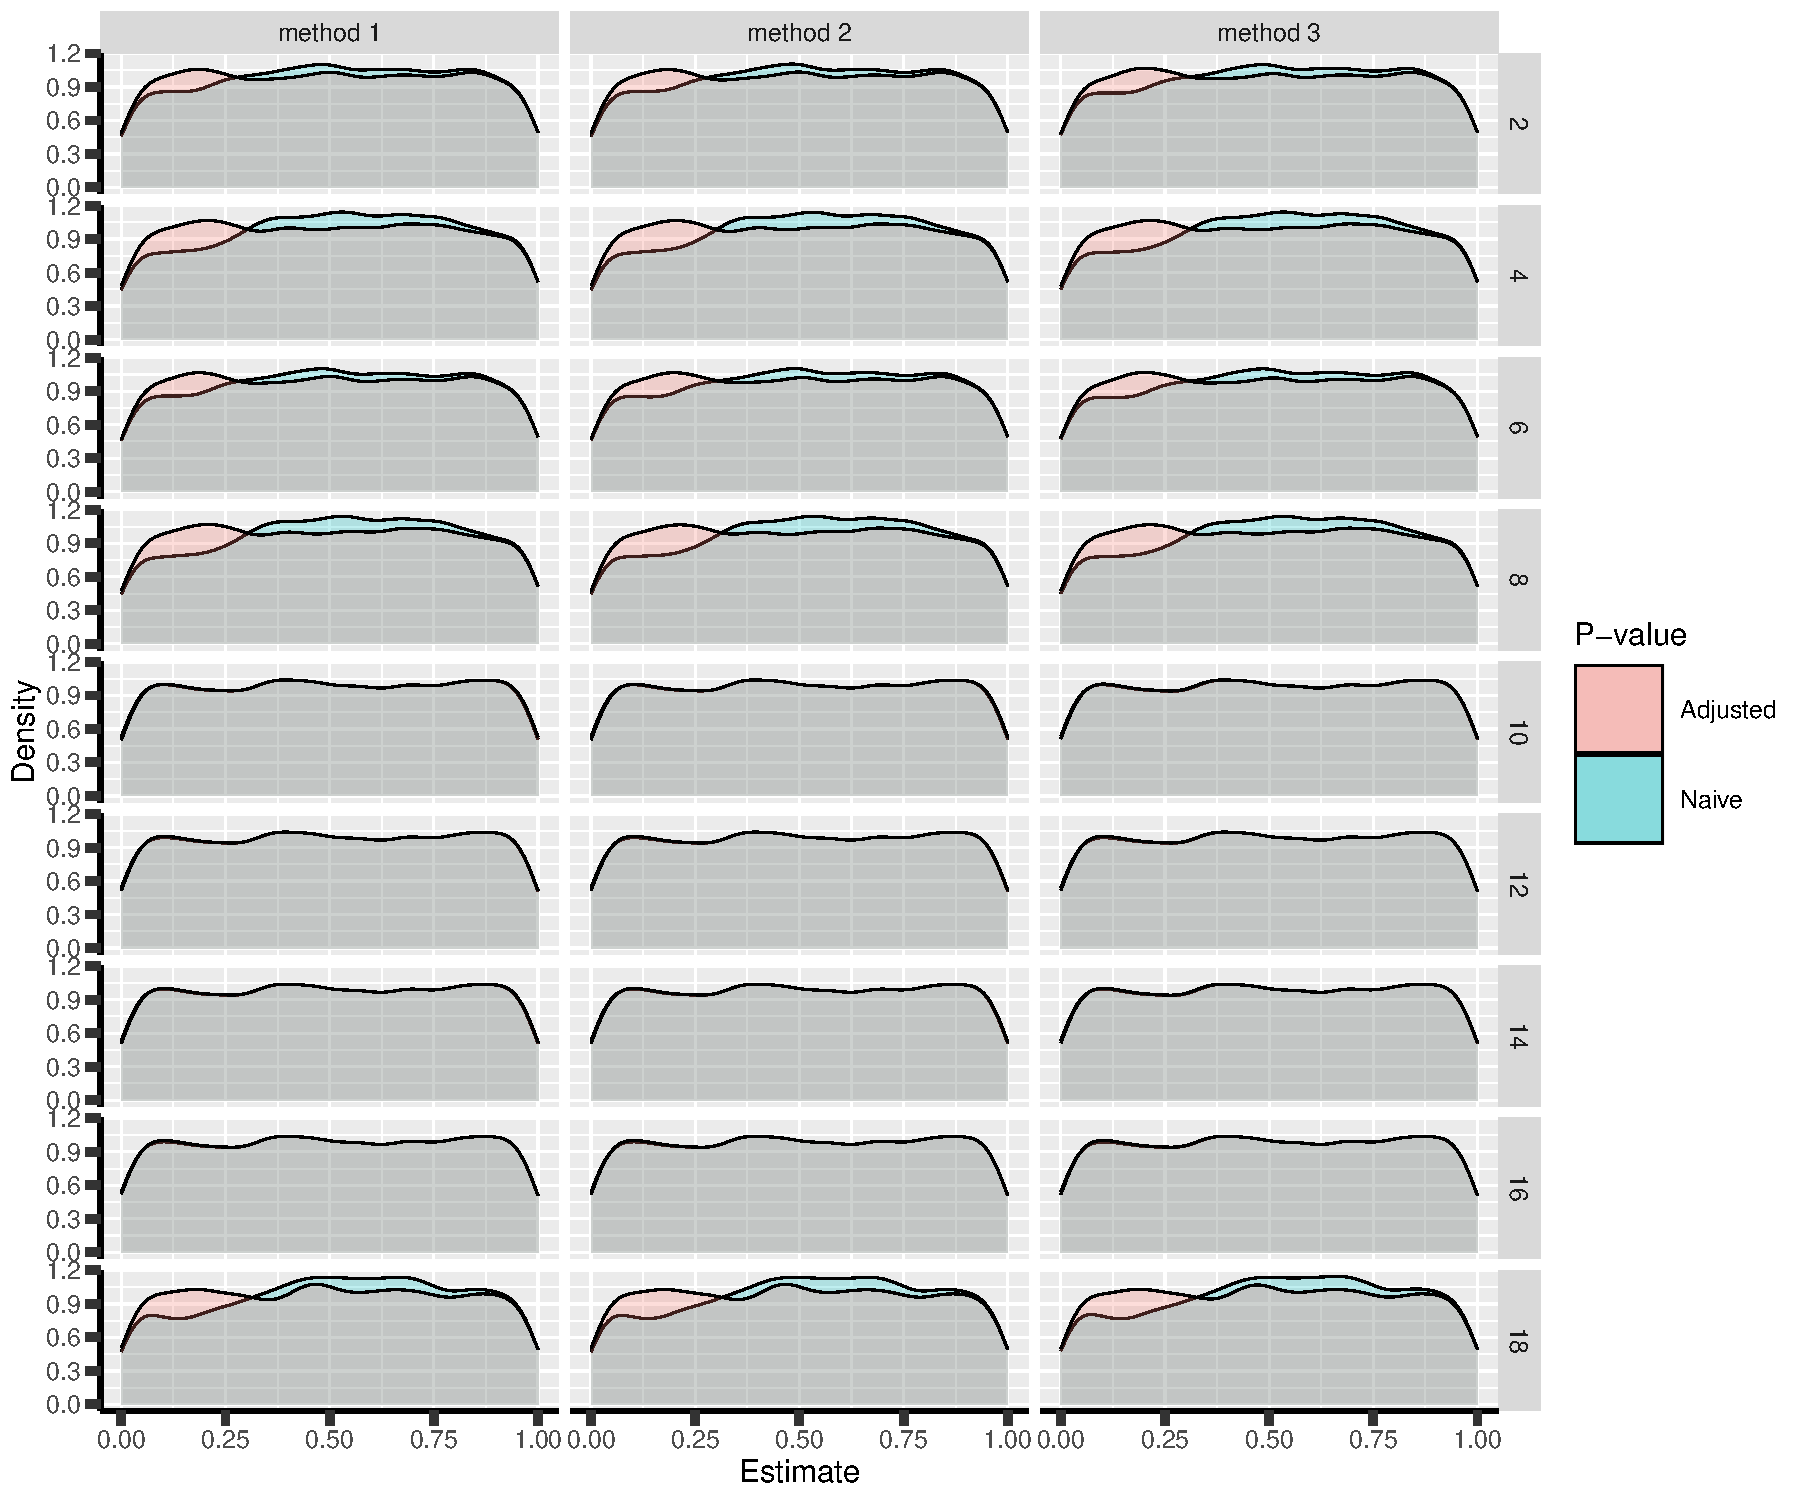
\includegraphics[trim={0 0 0 0},width=1\textwidth]{./figures/gg-pvalue-density.pdf}
\caption{Naive and adjusted p-value distribution over all simulations under the null. Each row correspond to a different scenario}
\end{figure}

\begin{figure}[!h]
\centering
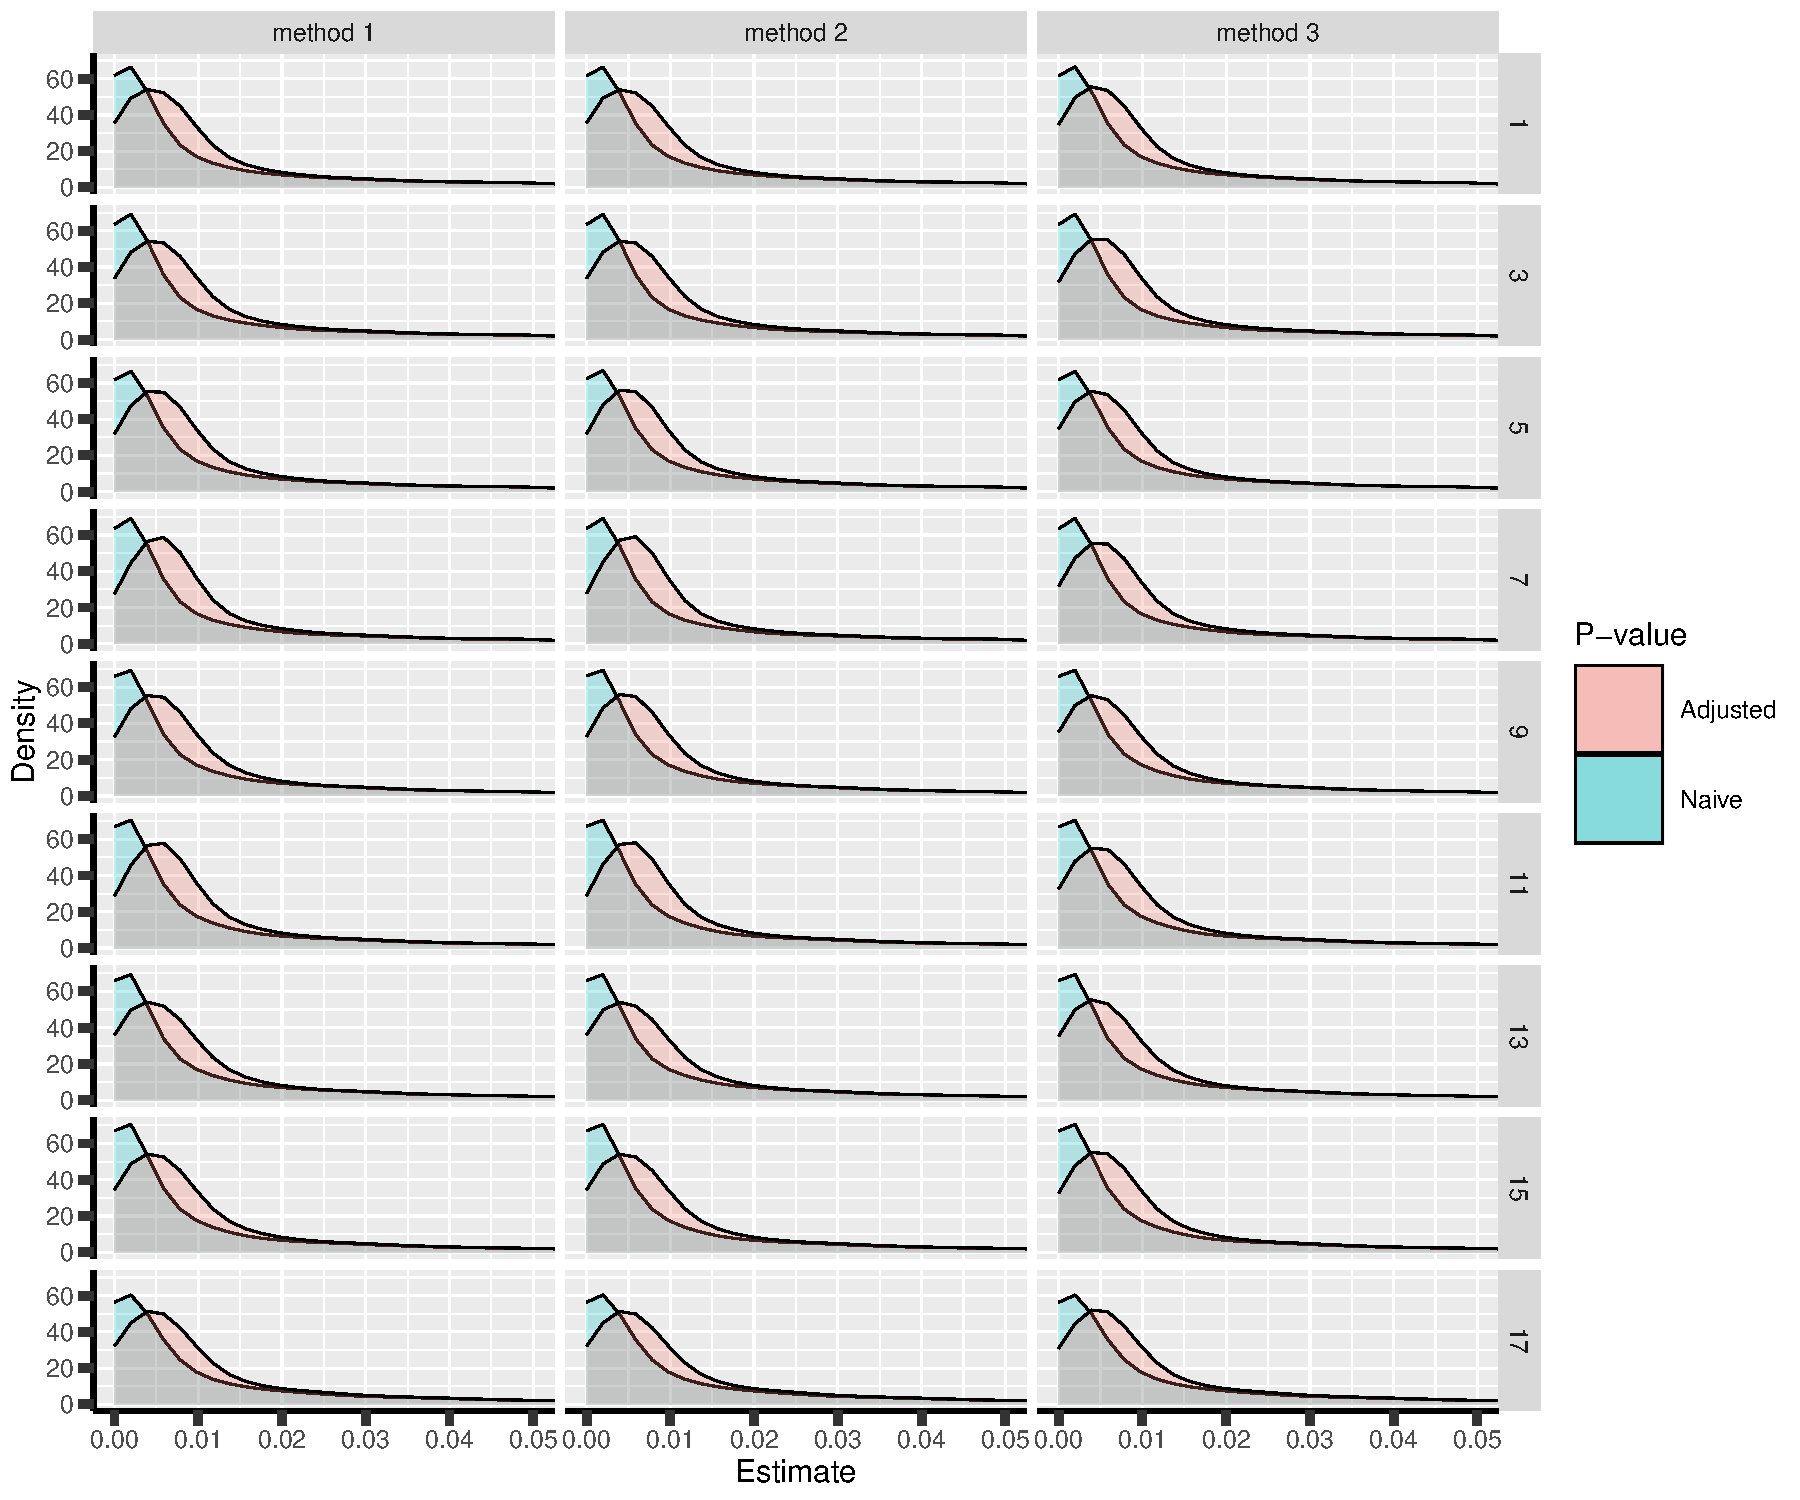
\includegraphics[trim={0 0 0 0},width=1\textwidth]{./figures/gg-pvalue2-density.pdf}
\caption{Naive and adjusted p-value distribution over all simulations under the alternative. Each row correspond to a different scenario}
\end{figure}

\clearpage

\section{Conclusion of the trial}
\label{sec:org08ef01f}

Relative frequency of stopping for efficacy/futility at decision/final

\begin{itemize}
\item Method 1
\end{itemize}
\begin{verbatim}
        N missing  hypo binding  fixC ar decision.eff decision.fut final.eff final.fut
 1: 10000    TRUE power    TRUE FALSE 10        37.82         6.05     43.18      13.0
 2: 10000    TRUE typeI    TRUE FALSE 10         0.79        70.85      1.67      26.7
 3: 10000    TRUE power    TRUE FALSE  5        35.60         6.02     45.00      13.4
 4: 10000    TRUE typeI    TRUE FALSE  5         0.68        69.21      1.74      28.4
 5: 10000    TRUE power    TRUE  TRUE 10        36.45         6.53     43.36      13.7
 6: 10000    TRUE typeI    TRUE  TRUE 10         0.64        71.29      1.61      26.5
 7: 10000    TRUE power    TRUE  TRUE  5        34.68         5.86     45.32      14.1
 8: 10000    TRUE typeI    TRUE  TRUE  5         0.72        69.11      1.70      28.5
 9: 10000    TRUE power   FALSE  TRUE 10        37.57         6.63     42.93      12.9
10: 10000    TRUE typeI   FALSE  TRUE 10         0.57         0.28      1.59      97.6
11: 10000    TRUE power   FALSE  TRUE  5        36.02         6.28     44.71      13.0
12: 10000    TRUE typeI   FALSE  TRUE  5         0.73         0.09      1.63      97.5
13: 10000    TRUE power   FALSE FALSE 10        38.32         5.87     42.35      13.5
14: 10000    TRUE typeI   FALSE FALSE 10         0.69         0.09      1.75      97.5
15: 10000    TRUE power   FALSE FALSE  5        36.75         5.70     43.90      13.6
16: 10000    TRUE typeI   FALSE FALSE  5         0.67         0.00      1.84      97.5
17: 10000   FALSE power    TRUE FALSE  5        33.98         5.33     46.33      14.4
18: 10000   FALSE typeI    TRUE FALSE  5         0.74        67.48      1.72      30.1
\end{verbatim}

\clearpage

Method 2:
\begin{verbatim}
        N missing  hypo binding  fixC ar decision.eff decision.fut final.eff final.fut
 1: 10000    TRUE power    TRUE FALSE 10        37.66         6.22     43.13      13.0
 2: 10000    TRUE typeI    TRUE FALSE 10         0.85        71.18      1.68      26.3
 3: 10000    TRUE power    TRUE FALSE  5        35.55         6.10     44.90      13.5
 4: 10000    TRUE typeI    TRUE FALSE  5         0.67        69.05      1.74      28.5
 5: 10000    TRUE power    TRUE  TRUE 10        36.82         5.94     43.59      13.6
 6: 10000    TRUE typeI    TRUE  TRUE 10         0.63        70.02      1.62      27.7
 7: 10000    TRUE power    TRUE  TRUE  5        35.06         5.63     45.40      13.9
 8: 10000    TRUE typeI    TRUE  TRUE  5         0.71        68.46      1.68      29.1
 9: 10000    TRUE power   FALSE  TRUE 10        37.76         6.21     43.09      12.9
10: 10000    TRUE typeI   FALSE  TRUE 10         0.56         0.26      1.62      97.6
11: 10000    TRUE power   FALSE  TRUE  5        36.07         6.10     44.75      13.1
12: 10000    TRUE typeI   FALSE  TRUE  5         0.72         0.07      1.63      97.6
13: 10000    TRUE power   FALSE FALSE 10        38.33         6.11     42.27      13.3
14: 10000    TRUE typeI   FALSE FALSE 10         0.69         0.09      1.75      97.5
15: 10000    TRUE power   FALSE FALSE  5        36.78         5.72     43.86      13.6
16: 10000    TRUE typeI   FALSE FALSE  5         0.66         0.01      1.84      97.5
17: 10000   FALSE power    TRUE FALSE  5        33.68         5.17     46.60      14.5
18: 10000   FALSE typeI    TRUE FALSE  5         0.72        67.42      1.72      30.1
\end{verbatim}

\clearpage

Method 3:
\begin{verbatim}
        N missing  hypo binding  fixC ar decision.eff decision.fut final.eff final.fut
 1: 10000    TRUE power    TRUE FALSE 10        40.44         6.54     40.01      13.0
 2: 10000    TRUE typeI    TRUE FALSE 10         0.74        68.77      1.66      28.8
 3: 10000    TRUE power    TRUE FALSE  5        36.49         6.42     43.72      13.4
 4: 10000    TRUE typeI    TRUE FALSE  5         0.68        68.37      1.72      29.2
 5: 10000    TRUE power    TRUE  TRUE 10        39.85         5.83     40.54      13.8
 6: 10000    TRUE typeI    TRUE  TRUE 10         0.73        68.89      1.72      28.7
 7: 10000    TRUE power    TRUE  TRUE  5        35.70         5.81     44.38      14.1
 8: 10000    TRUE typeI    TRUE  TRUE  5         0.78        68.26      1.72      29.2
 9: 10000    TRUE power   FALSE  TRUE 10        41.03         6.39     39.88      12.7
10: 10000    TRUE typeI   FALSE  TRUE 10         0.72         0.38      1.59      97.3
11: 10000    TRUE power   FALSE  TRUE  5        37.08         6.14     43.67      13.1
12: 10000    TRUE typeI   FALSE  TRUE  5         0.74         0.14      1.64      97.5
13: 10000    TRUE power   FALSE FALSE 10        41.47         6.05     39.18      13.3
14: 10000    TRUE typeI   FALSE FALSE 10         0.81         0.31      1.77      97.1
15: 10000    TRUE power   FALSE FALSE  5        37.37         5.86     43.09      13.7
16: 10000    TRUE typeI   FALSE FALSE  5         0.75         0.08      1.83      97.3
17: 10000   FALSE power    TRUE FALSE  5        34.66         5.58     45.27      14.5
18: 10000   FALSE typeI    TRUE FALSE  5         0.68        66.54      1.77      31.0
\end{verbatim}

\clearpage

\section{Bias (True effect: 0.6 under the alternative)}
\label{sec:orgb253994}

Bias per estimator and method\footnote{e.g. \texttt{biasMLE1} mixed model
estimator (treatment effect), method 1 (boundaries)}:
\begin{adjustwidth}{-1cm}{-1cm}
\begin{verbatim}
     hypo missing binding  fixC ar  biasMLE1  biasMLE2  biasMLE3  biasMUE1  biasMUE2  biasMUE3
 1: power    TRUE    TRUE FALSE 10  0.012970  0.013058  0.014139  5.47e-03  5.56e-03  0.001778
 2: typeI    TRUE    TRUE FALSE 10 -0.018416 -0.018430 -0.018509 -4.26e-03 -4.33e-03 -0.004919
 3: power    TRUE    TRUE FALSE  5  0.022430  0.022231  0.023386  1.01e-02  1.02e-02  0.008425
 4: typeI    TRUE    TRUE FALSE  5 -0.030419 -0.030822 -0.030577 -1.18e-02 -1.21e-02 -0.012275
 5: power    TRUE    TRUE  TRUE 10  0.011558  0.012119  0.012968 -1.55e-04  8.16e-04  0.001723
 6: typeI    TRUE    TRUE  TRUE 10 -0.022074 -0.022256 -0.022266 -9.04e-03 -9.08e-03 -0.008580
 7: power    TRUE    TRUE  TRUE  5  0.021638  0.022029  0.022692  7.84e-03  8.10e-03  0.008201
 8: typeI    TRUE    TRUE  TRUE  5 -0.033857 -0.034379 -0.034138 -1.50e-02 -1.51e-02 -0.015168
 9: power    TRUE   FALSE  TRUE 10  0.015026  0.015050  0.016312 -7.62e-04 -4.88e-04  0.000843
10: typeI    TRUE   FALSE  TRUE 10  0.000543  0.000547  0.000883 -6.54e-05 -1.08e-06  0.001751
11: power    TRUE   FALSE  TRUE  5  0.024204  0.024192  0.025190  6.44e-03  5.95e-03  0.007381
12: typeI    TRUE   FALSE  TRUE  5  0.001472  0.001451  0.001545  1.17e-03  1.21e-03  0.001552
13: power    TRUE   FALSE FALSE 10  0.014415  0.014146  0.015747  3.10e-03  2.68e-03  0.002008
14: typeI    TRUE   FALSE FALSE 10  0.000139  0.000139  0.000555 -1.53e-05 -2.18e-05  0.001472
15: power    TRUE   FALSE FALSE  5  0.023380  0.023344  0.024346  8.80e-03  8.79e-03  0.007463
16: typeI    TRUE   FALSE FALSE  5  0.000602  0.000602  0.000949  5.40e-04  5.00e-04  0.001079
17: power   FALSE    TRUE FALSE  5  0.022836  0.022825  0.023807  1.20e-02  1.21e-02  0.010058
18: typeI   FALSE    TRUE FALSE  5 -0.029516 -0.029722 -0.029915 -1.10e-02 -1.14e-02 -0.011615
\end{verbatim}
\end{adjustwidth}

Median bias \footnote{Relative frequency at which the estimate is greater than the truth minus 0.5} per estimator and method:
\begin{adjustwidth}{-1cm}{-1cm}
\begin{verbatim}
     hypo missing binding  fixC ar mbiasMLE1 mbiasMLE2 mbiasMLE3 mbiasMUE1 mbiasMUE2 mbiasMUE3
 1: power    TRUE    TRUE FALSE 10    0.0250    0.0240    0.0266   -0.0023   -0.0017   -0.0062
 2: typeI    TRUE    TRUE FALSE 10   -0.0193   -0.0198   -0.0223    0.0002   -0.0013    0.0001
 3: power    TRUE    TRUE FALSE  5    0.0387    0.0382    0.0406   -0.0030   -0.0016   -0.0026
 4: typeI    TRUE    TRUE FALSE  5   -0.0346   -0.0339   -0.0361    0.0000   -0.0002    0.0001
 5: power    TRUE    TRUE  TRUE 10    0.0164    0.0188    0.0179   -0.0134   -0.0128   -0.0102
 6: typeI    TRUE    TRUE  TRUE 10   -0.0327   -0.0314   -0.0347   -0.0113   -0.0079   -0.0099
 7: power    TRUE    TRUE  TRUE  5    0.0356    0.0369    0.0361   -0.0106   -0.0115   -0.0082
 8: typeI    TRUE    TRUE  TRUE  5   -0.0473   -0.0492   -0.0493   -0.0105   -0.0081   -0.0105
 9: power    TRUE   FALSE  TRUE 10    0.0328    0.0301    0.0345   -0.0092   -0.0110   -0.0055
10: typeI    TRUE   FALSE  TRUE 10    0.0007   -0.0019    0.0007    0.0008   -0.0018    0.0030
11: power    TRUE   FALSE  TRUE  5    0.0479    0.0459    0.0499   -0.0049   -0.0049   -0.0034
12: typeI    TRUE   FALSE  TRUE  5    0.0009   -0.0017    0.0009    0.0009   -0.0017    0.0013
13: power    TRUE   FALSE FALSE 10    0.0326    0.0324    0.0339   -0.0033   -0.0036   -0.0005
14: typeI    TRUE   FALSE FALSE 10   -0.0039   -0.0039   -0.0037   -0.0039   -0.0039   -0.0015
15: power    TRUE   FALSE FALSE  5    0.0442    0.0442    0.0465   -0.0010   -0.0010   -0.0038
16: typeI    TRUE   FALSE FALSE  5   -0.0039   -0.0039   -0.0039   -0.0039   -0.0039   -0.0031
17: power   FALSE    TRUE FALSE  5    0.0383    0.0378    0.0400   -0.0026   -0.0008   -0.0046
18: typeI   FALSE    TRUE FALSE  5   -0.0329   -0.0336   -0.0353    0.0044    0.0031    0.0035
\end{verbatim}

\end{adjustwidth}

\clearpage

\section{Distribution of the estimates}
\label{sec:org739ac20}

Distribution of the estimates:
\begin{figure}[!h]
\centering
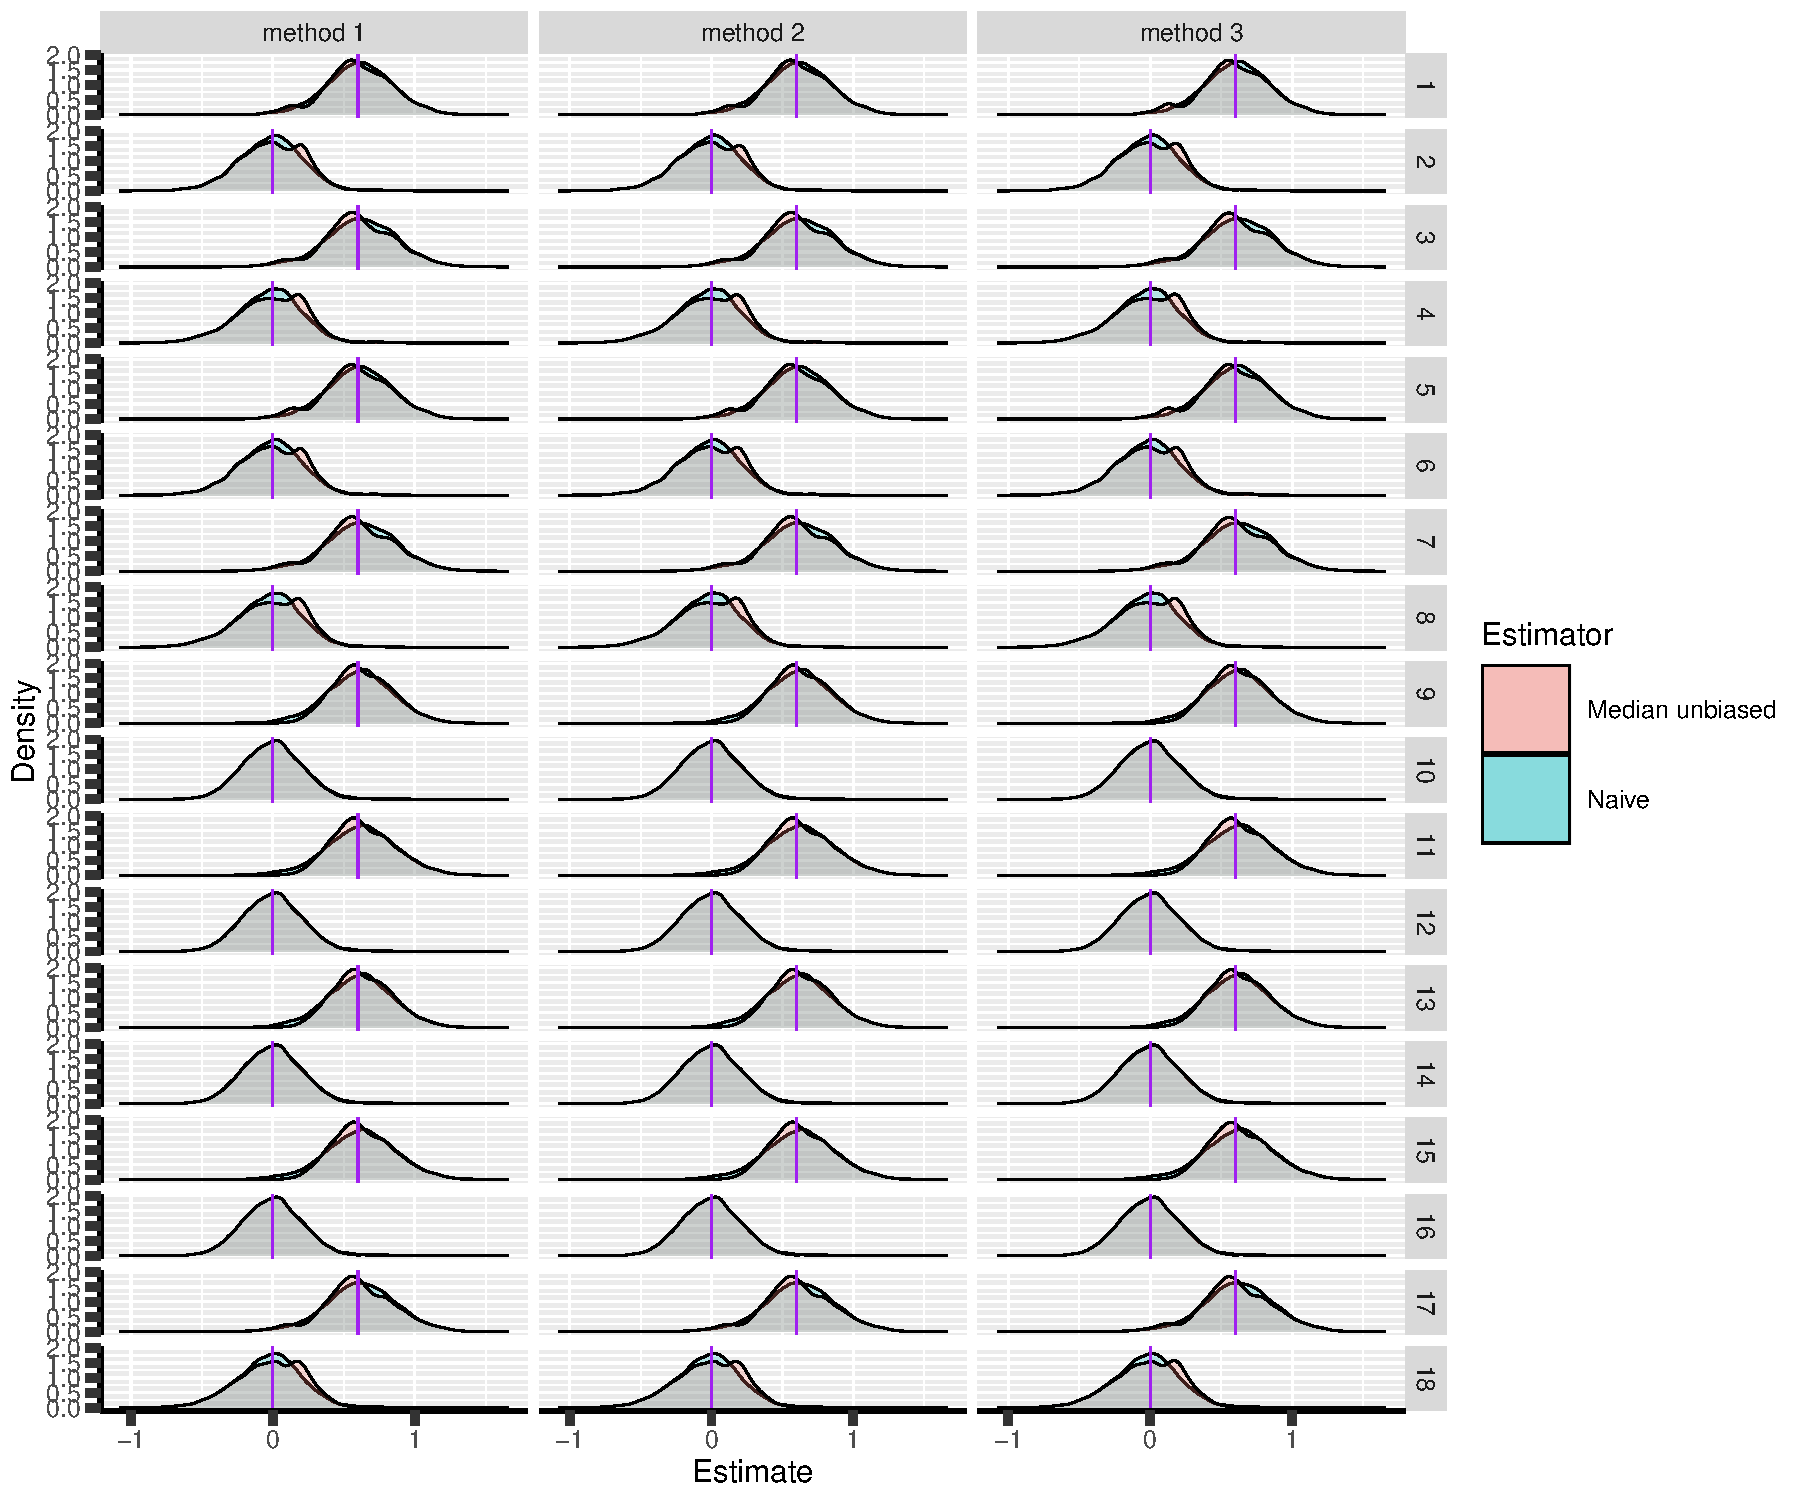
\includegraphics[trim={0 0 0 0},width=1\textwidth]{./figures/gg-estimate-density.pdf}
\caption{Naive and Median unbiased estimate distribution over all simulations. Each row correspond to a different scenario}
\end{figure}

\begin{figure}[!h]
\centering
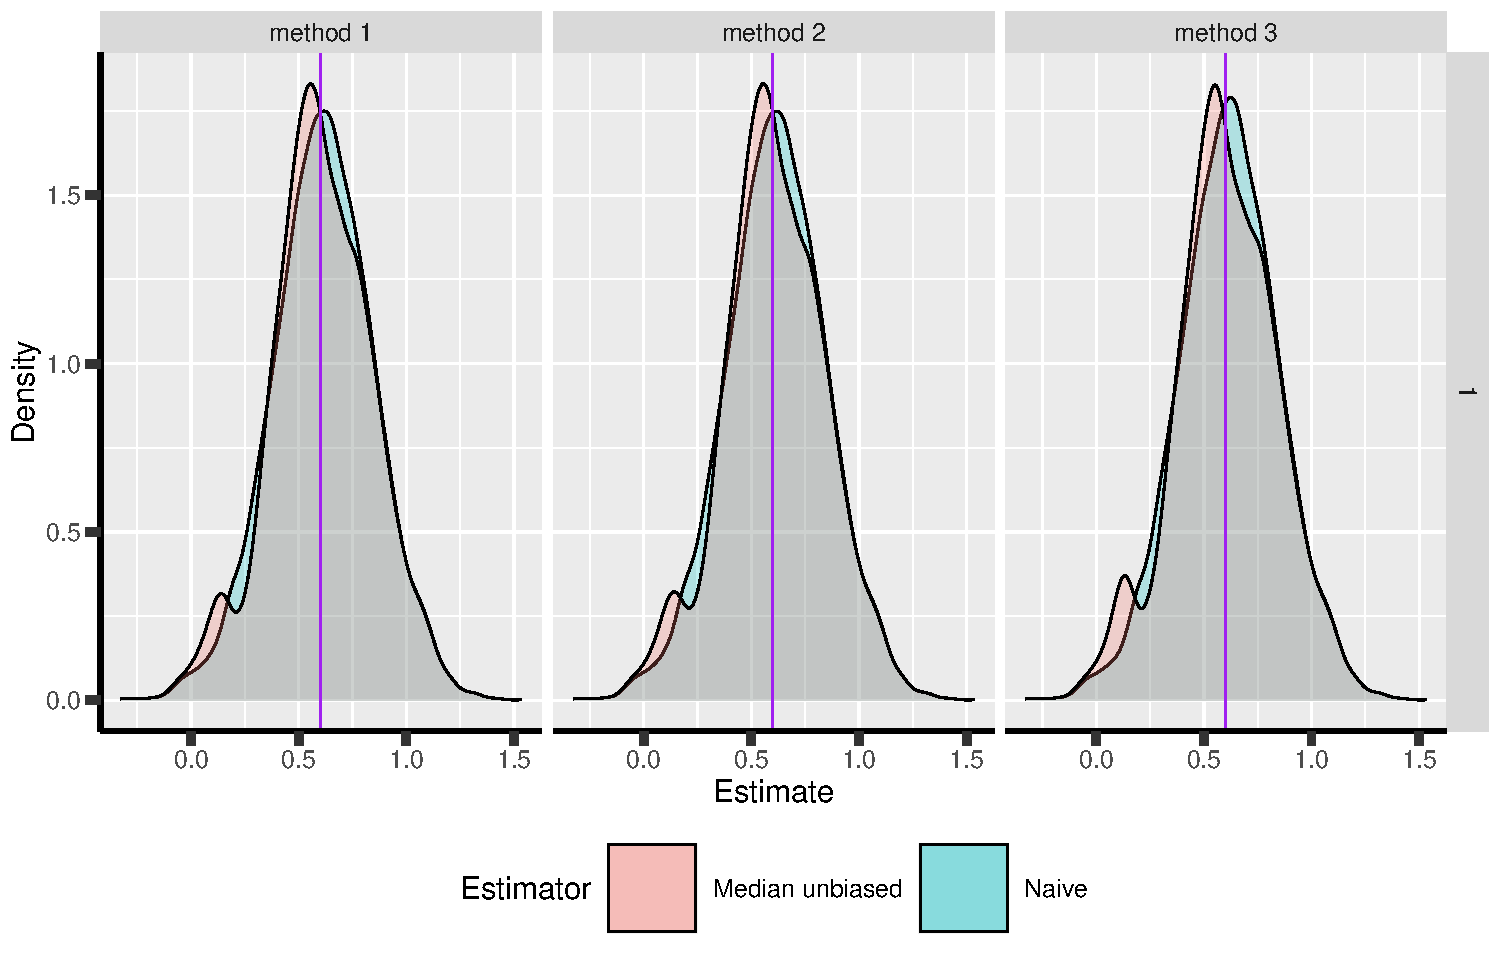
\includegraphics[trim={0 0 0 0},width=\textwidth]{./figures/gg-estimate-density-scenario1.pdf}
\caption{Same but specific to scenario 1}
\end{figure}

\clearpage

Distribution of the median unbiased estimate conditional to the stage:
\begin{figure}[!h]
\centering
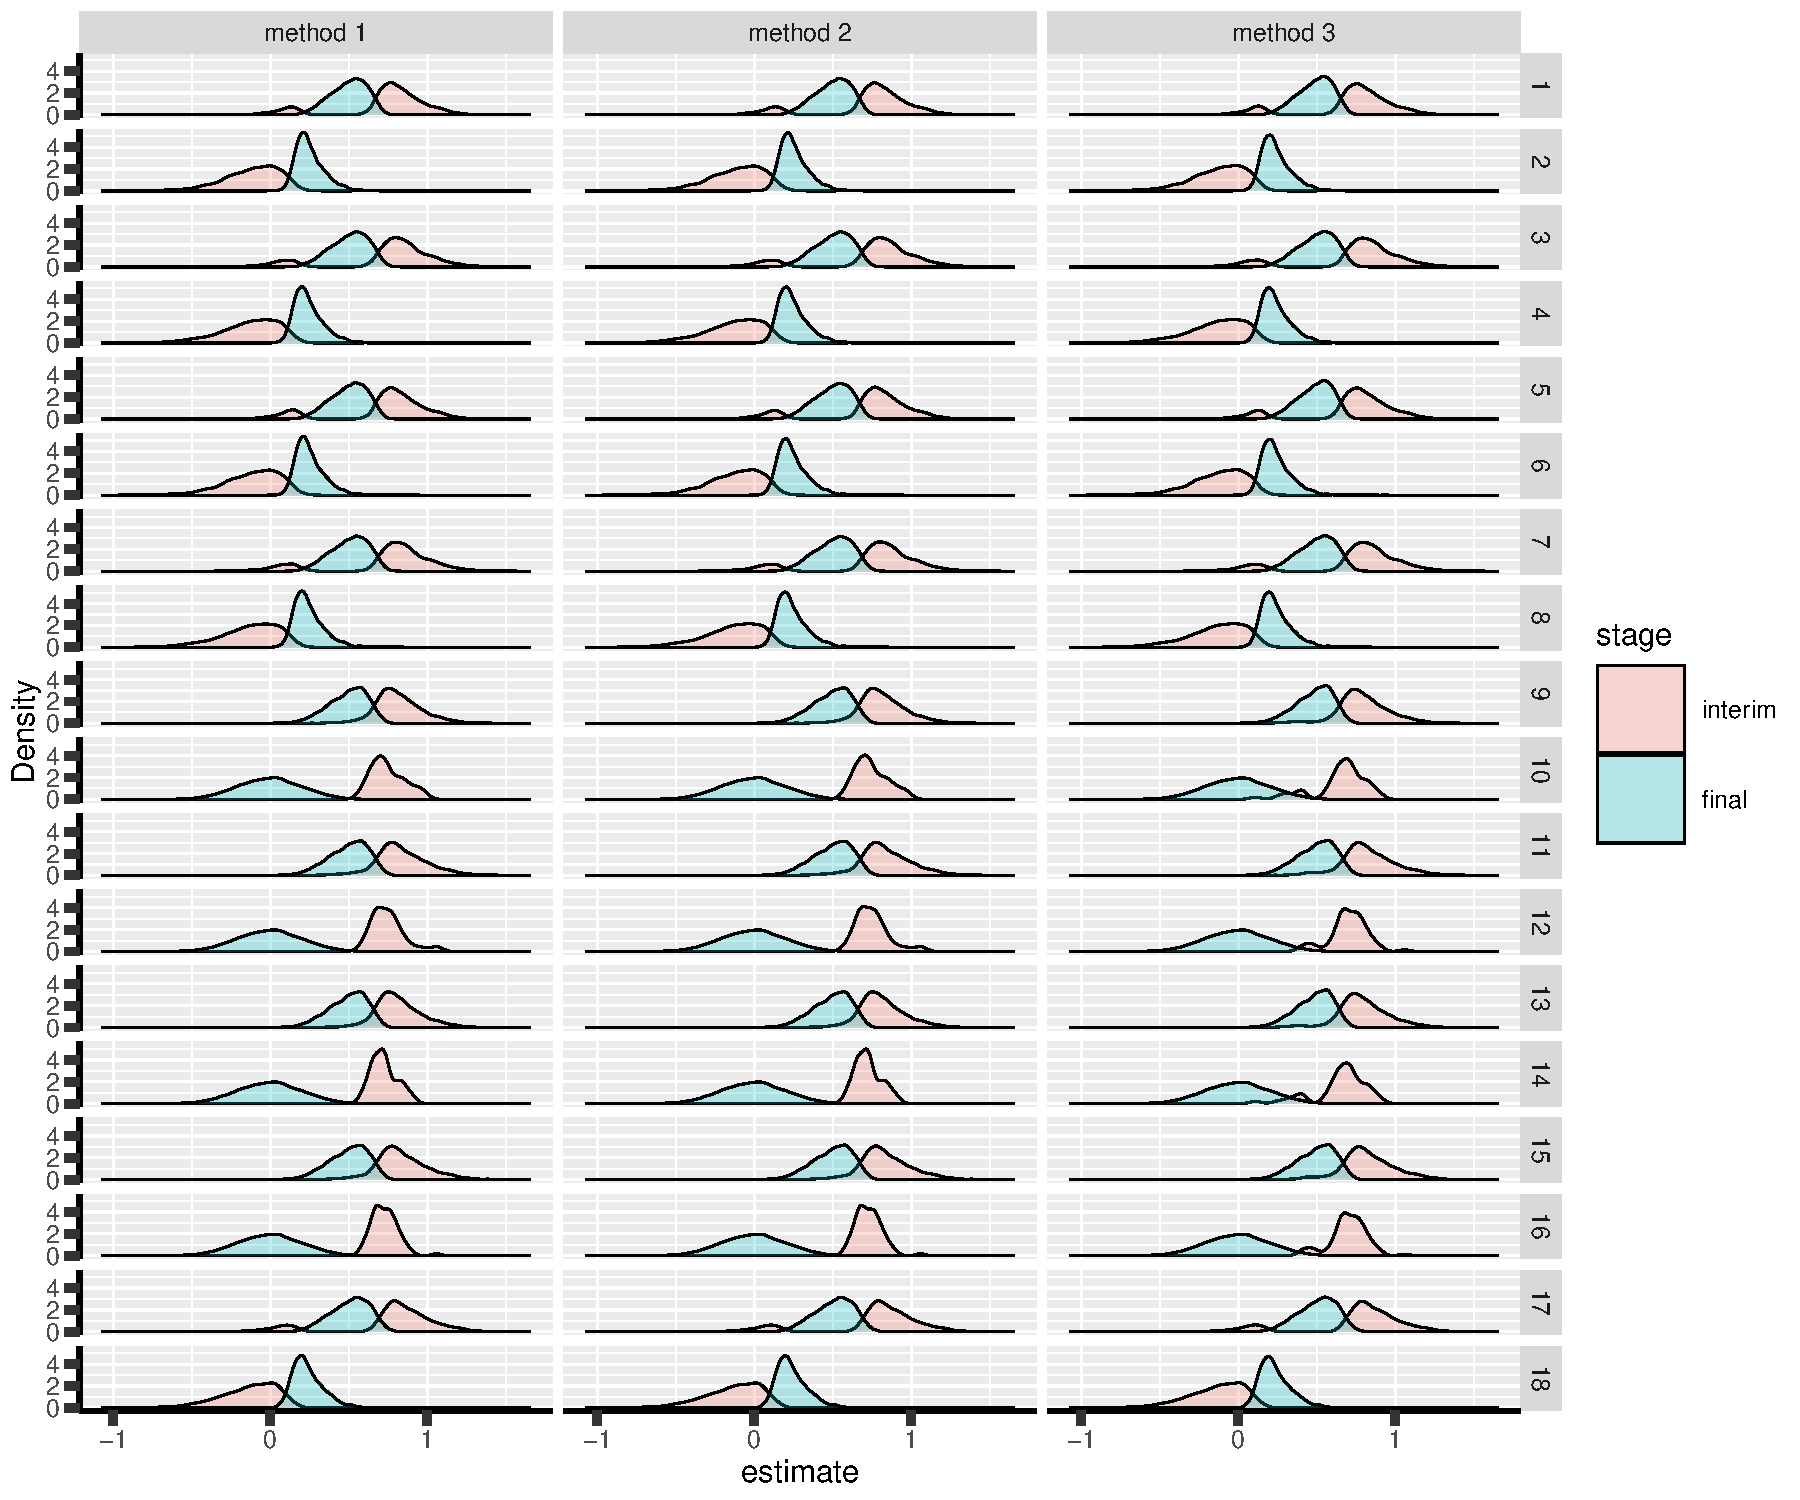
\includegraphics[trim={0 0 0 0},width=1\textwidth]{./figures/gg-estimateC-density.pdf}
\caption{Median unbiased estimate distribution conditional to the stage. Each row correspond to a different scenario.}
\end{figure}

\clearpage

\section{Special cases}
\label{sec:org2bc044e}

Reason for stopping (first 4) or continuing the trial (last):
\begin{verbatim}
                              scenario    1    2    3    4    5    6    7    8
reason                 method                                                 
decreasing information 1                  0    0    1    1    0    0    0    0
                       2                  0    0    1    1    0    0    0    0
                       3                  0    0    1    1    0    0    0    0
efficacy               1               3740   77 3559   67 3696   82 3502   82
                       2               3729   82 3554   68 3732   82 3546   83
                       3               4137  107 3712   83 4071  110 3632   92
futility               1                646 7086  603 6922  600 7109  552 6901
                       2                658 7120  611 6904  542 6981  523 6834
                       3                560 6843  579 6822  495 6850  519 6812
Imax reached           1                  1    1    0    0    2    2    0    0
                       2                  1    1    0    0    2    2    0    0
                       3                  1    1    0    0    2    2    0    0
no boundary crossed    1               5613 2836 5838 3011 5702 2807 5946 3017
                       2               5612 2797 5835 3028 5724 2935 5931 3083
                       3               5302 3049 5709 3095 5432 3038 5849 3096
\end{verbatim}

\begin{verbatim}
                              scenario    9   10   11   12   13   14   15   16
reason                 method                                                 
decreasing information 1                  0    0    1    0    0    0    0    0
                       2                  0    0    1    0    0    0    0    0
                       3                  0    0    1    0    0    0    0    0
efficacy               1               3805   84 3634   82 3815   78 3674   67
                       2               3824   81 3646   79 3816   78 3677   67
                       3               4206  109 3761   88 4238  112 3788   83
futility               1                614 7130  596 6957  604 7126  571 6920
                       2                572 7044  571 6907  628 7180  573 6925
                       3                535 6914  561 6867  514 6870  535 6837
Imax reached           1                  1    1    0    0    0    0    0    0
                       2                  1    1    0    0    0    0    0    0
                       3                  1    1    0    0    0    0    0    0
no boundary crossed    1               5580 2785 5770 2961 5581 2796 5755 3013
                       2               5603 2874 5783 3014 5556 2742 5750 3008
                       3               5258 2976 5678 3045 5248 3018 5677 3080
\end{verbatim}

\clearpage

\section{Reversal probability}
\label{sec:org7975a08}

Percentage of time we observe a reversal:
\begin{adjustwidth}{-1cm}{-1cm}
\begin{verbatim}
        N  hypo missing ar binding  fixC fu2eff_1 fu2eff_2 fu2eff_3 eff2fu_1 eff2fu_2 eff2fu_3
 1: 10000 power   FALSE  5    TRUE FALSE     0.06     0.07     0.01     0.04     0.04     0.63
 2: 10000 power    TRUE  5   FALSE FALSE     0.04     0.04     0.00     0.03     0.03     0.51
 3: 10000 power    TRUE  5   FALSE  TRUE     0.04     0.03     0.03     0.36     0.42     0.56
 4: 10000 power    TRUE  5    TRUE FALSE     0.06     0.08     0.02     0.05     0.07     0.65
 5: 10000 power    TRUE  5    TRUE  TRUE     0.02     0.02     0.01     0.36     0.42     0.63
 6: 10000 power    TRUE 10   FALSE FALSE     0.35     0.38     0.05     0.18     0.21     0.96
 7: 10000 power    TRUE 10   FALSE  TRUE     0.15     0.13     0.10     0.63     0.61     1.13
 8: 10000 power    TRUE 10    TRUE FALSE     0.57     0.57     0.13     0.15     0.20     1.06
 9: 10000 power    TRUE 10    TRUE  TRUE     0.17     0.16     0.11     0.70     0.68     0.99
10: 10000 typeI   FALSE  5    TRUE FALSE     0.01     0.03     0.00     0.01     0.03     0.12
11: 10000 typeI    TRUE  5   FALSE FALSE     0.00     0.00     0.00     0.00     0.01     0.08
12: 10000 typeI    TRUE  5   FALSE  TRUE     0.00     0.00     0.00     0.09     0.07     0.14
13: 10000 typeI    TRUE  5    TRUE FALSE     0.02     0.02     0.00     0.01     0.03     0.15
14: 10000 typeI    TRUE  5    TRUE  TRUE     0.00     0.00     0.00     0.10     0.12     0.14
15: 10000 typeI    TRUE 10   FALSE FALSE     0.00     0.00     0.00     0.09     0.09     0.31
16: 10000 typeI    TRUE 10   FALSE  TRUE     0.00     0.00     0.00     0.27     0.25     0.37
17: 10000 typeI    TRUE 10    TRUE FALSE     0.11     0.11     0.03     0.09     0.08     0.36
18: 10000 typeI    TRUE 10    TRUE  TRUE     0.02     0.00     0.00     0.22     0.21     0.39
\end{verbatim}

\end{adjustwidth}


\clearpage

\section{Frequency mismatch}
\label{sec:org49bce0d}

\subsection{p-value / boundaries}
\label{sec:orgd89305d}

When concluding for futility:
\begin{verbatim}
     hypo missing ar binding  fixC method 1 method 2 method 3
 1: power   FALSE  5    TRUE FALSE        0        0        0
 2: power    TRUE  5   FALSE FALSE        0        0        0
 3: power    TRUE  5   FALSE  TRUE        0        0        0
 4: power    TRUE  5    TRUE FALSE        0        0        0
 5: power    TRUE  5    TRUE  TRUE        0        0        0
 6: power    TRUE 10   FALSE FALSE        0        0        0
 7: power    TRUE 10   FALSE  TRUE        0        0        0
 8: power    TRUE 10    TRUE FALSE        0        0        0
 9: power    TRUE 10    TRUE  TRUE        0        0        0
10: typeI   FALSE  5    TRUE FALSE        0        0        0
11: typeI    TRUE  5   FALSE FALSE        0        0        0
12: typeI    TRUE  5   FALSE  TRUE        0        0        0
13: typeI    TRUE  5    TRUE FALSE        0        0        0
14: typeI    TRUE  5    TRUE  TRUE        0        0        0
15: typeI    TRUE 10   FALSE FALSE        0        0        0
16: typeI    TRUE 10   FALSE  TRUE        0        0        0
17: typeI    TRUE 10    TRUE FALSE        0        0        0
18: typeI    TRUE 10    TRUE  TRUE        0        0        0
\end{verbatim}

When concluding for efficacy:
\begin{verbatim}
     hypo missing ar binding  fixC method 1 method 2 method 3
 1: power   FALSE  5    TRUE FALSE        0        0        0
 2: power    TRUE  5   FALSE FALSE        0        0        0
 3: power    TRUE  5   FALSE  TRUE        0        0        0
 4: power    TRUE  5    TRUE FALSE        0        0        0
 5: power    TRUE  5    TRUE  TRUE        0        0        0
 6: power    TRUE 10   FALSE FALSE        0        0        0
 7: power    TRUE 10   FALSE  TRUE        0        0        0
 8: power    TRUE 10    TRUE FALSE        0        0        0
 9: power    TRUE 10    TRUE  TRUE        0        0        0
10: typeI   FALSE  5    TRUE FALSE        0        0        0
11: typeI    TRUE  5   FALSE FALSE        0        0        0
12: typeI    TRUE  5   FALSE  TRUE        0        0        0
13: typeI    TRUE  5    TRUE FALSE        0        0        0
14: typeI    TRUE  5    TRUE  TRUE        0        0        0
15: typeI    TRUE 10   FALSE FALSE        0        0        0
16: typeI    TRUE 10   FALSE  TRUE        0        0        0
17: typeI    TRUE 10    TRUE FALSE        0        0        0
18: typeI    TRUE 10    TRUE  TRUE        0        0        0
\end{verbatim}

\clearpage

\subsection{confidence intervals}
\label{sec:orgad7b21f}

When concluding for futility:
\begin{verbatim}
     hypo missing ar binding  fixC   method 1   method 2   method 3
 1: power   FALSE  5    TRUE FALSE 0.00000000 0.00000000 0.00000000
 2: power    TRUE  5   FALSE FALSE 0.00000000 0.00000000 0.00000000
 3: power    TRUE  5   FALSE  TRUE 0.05189414 0.05213764 0.05194805
 4: power    TRUE  5    TRUE FALSE 0.00000000 0.00000000 0.00000000
 5: power    TRUE  5    TRUE  TRUE 0.00000000 0.00000000 0.00000000
 6: power    TRUE 10   FALSE FALSE 0.00000000 0.00000000 0.00000000
 7: power    TRUE 10   FALSE  TRUE 0.05128205 0.05221932 0.05238345
 8: power    TRUE 10    TRUE FALSE 0.05263158 0.05205622 0.05115090
 9: power    TRUE 10    TRUE  TRUE 0.00000000 0.00000000 0.00000000
10: typeI   FALSE  5    TRUE FALSE 2.46052901 2.41902419 2.46027678
11: typeI    TRUE  5   FALSE FALSE 2.54385065 2.54358974 1.89899405
12: typeI    TRUE  5   FALSE  TRUE 2.63211798 2.63184844 1.92583487
13: typeI    TRUE  5    TRUE FALSE 2.94117647 2.87939338 2.94057377
14: typeI    TRUE  5    TRUE  TRUE 2.58249641 2.42802991 2.58461538
15: typeI    TRUE 10   FALSE FALSE 2.54202542 2.54202542 1.26257442
16: typeI    TRUE 10   FALSE  TRUE 2.62673753 2.62727459 1.23861194
17: typeI    TRUE 10    TRUE FALSE 2.73733853 2.71878527 2.73565574
18: typeI    TRUE 10    TRUE  TRUE 2.47570332 2.51662404 2.48077909
\end{verbatim}

When concluding for efficacy:
\begin{verbatim}
     hypo missing ar binding  fixC method 1 method 2 method 3
 1: power   FALSE  5    TRUE FALSE        0        0        0
 2: power    TRUE  5   FALSE FALSE        0        0        0
 3: power    TRUE  5   FALSE  TRUE        0        0        0
 4: power    TRUE  5    TRUE FALSE        0        0        0
 5: power    TRUE  5    TRUE  TRUE        0        0        0
 6: power    TRUE 10   FALSE FALSE        0        0        0
 7: power    TRUE 10   FALSE  TRUE        0        0        0
 8: power    TRUE 10    TRUE FALSE        0        0        0
 9: power    TRUE 10    TRUE  TRUE        0        0        0
10: typeI   FALSE  5    TRUE FALSE        0        0        0
11: typeI    TRUE  5   FALSE FALSE        0        0        0
12: typeI    TRUE  5   FALSE  TRUE        0        0        0
13: typeI    TRUE  5    TRUE FALSE        0        0        0
14: typeI    TRUE  5    TRUE  TRUE        0        0        0
15: typeI    TRUE 10   FALSE FALSE        0        0        0
16: typeI    TRUE 10   FALSE  TRUE        0        0        0
17: typeI    TRUE 10    TRUE FALSE        0        0        0
18: typeI    TRUE 10    TRUE  TRUE        0        0        0
\end{verbatim}

\section{Coverage}
\label{sec:orgfe83495}

Average width of the confidence intervals
\lstset{language=r,label= ,caption= ,captionpos=b,numbers=none}
\begin{lstlisting}
res2stage.width <- res2stage[decision %in% c("futility","efficacy"),
                             .(N = .N,
                               width.naive = mean(upper_ML-lower_ML),
                               width.MUE = mean(upper_MUE-lower_MUE)),
                             by = c("method.char","missing","binding","fixC","ar","hypo")]
res2stage.width[, width.ratio := width.MUE/width.naive]
dcast(res2stage.width, hypo + missing + ar + binding + fixC ~ method.char, value.var = "width.ratio")
\end{lstlisting}

\begin{verbatim}
     hypo missing ar binding  fixC  method 1  method 2 method 3
 1: power   FALSE  5    TRUE FALSE 1.0517981 1.0518767 1.053589
 2: power    TRUE  5   FALSE FALSE 1.0430641 1.0430645 1.045294
 3: power    TRUE  5   FALSE  TRUE 1.0490757 1.0494445 1.045526
 4: power    TRUE  5    TRUE FALSE 1.0516795 1.0515698 1.052909
 5: power    TRUE  5    TRUE  TRUE 1.0580807 1.0575936 1.054137
 6: power    TRUE 10   FALSE FALSE 1.0532980 1.0532804 1.055866
 7: power    TRUE 10   FALSE  TRUE 1.0679703 1.0676474 1.056350
 8: power    TRUE 10    TRUE FALSE 1.0625603 1.0625641 1.062728
 9: power    TRUE 10    TRUE  TRUE 1.0774122 1.0766805 1.063708
10: typeI   FALSE  5    TRUE FALSE 1.0431774 1.0434979 1.046821
11: typeI    TRUE  5   FALSE FALSE 0.9994186 0.9994094 1.019993
12: typeI    TRUE  5   FALSE  TRUE 0.9994042 0.9994106 1.020071
13: typeI    TRUE  5    TRUE FALSE 1.0417925 1.0419051 1.045259
14: typeI    TRUE  5    TRUE  TRUE 1.0424393 1.0429751 1.045768
15: typeI    TRUE 10   FALSE FALSE 0.9946568 0.9949442 1.052180
16: typeI    TRUE 10   FALSE  TRUE 0.9951513 0.9954542 1.051935
17: typeI    TRUE 10    TRUE FALSE 1.0462148 1.0458686 1.056152
18: typeI    TRUE 10    TRUE  TRUE 1.0462813 1.0476594 1.056027
\end{verbatim}

\section{Percentage of missing values}
\label{sec:orga0e8a8d}

Here only for method 1 - values are very similar between different
methods:
\begin{itemize}
\item \texttt{pc.all} percentage of observations with full data
\item \texttt{pc.missing3} percentage of observations missing the final outcome
but with intermediate outcome value and baseline.
\item \texttt{pc.missing23} percentage of observations with only baseline value
\end{itemize}
\begin{verbatim}
    method missing ar  hypo  fixC binding     N   pc.all pc.missing3 pc.missing23
 1:      1    TRUE  5 power FALSE    TRUE 10000 79.53472    9.562374    10.902910
 2:      1    TRUE  5 typeI FALSE    TRUE 10000 79.53472    9.562374    10.902910
 3:      1    TRUE  5 power  TRUE    TRUE 10000 79.44022    9.531225    11.028558
 4:      1    TRUE  5 typeI  TRUE    TRUE 10000 79.44022    9.531225    11.028558
 5:      1    TRUE  5 power  TRUE   FALSE 10000 79.71917    9.427430    10.853396
 6:      1    TRUE  5 typeI  TRUE   FALSE 10000 79.71917    9.427430    10.853396
 7:      1    TRUE  5 power FALSE   FALSE 10000 79.64196    9.449136    10.908902
 8:      1    TRUE  5 typeI FALSE   FALSE 10000 79.64196    9.449136    10.908902
 9:      1   FALSE  5 power FALSE    TRUE 10000 87.78863    6.090240     6.121126
10:      1   FALSE  5 typeI FALSE    TRUE 10000 87.78863    6.090240     6.121126
11:      1    TRUE 10 power FALSE    TRUE 10000 71.60971   13.327969    15.062319
12:      1    TRUE 10 typeI FALSE    TRUE 10000 71.60971   13.327969    15.062319
13:      1    TRUE 10 power  TRUE    TRUE 10000 71.52189   13.282615    15.195496
14:      1    TRUE 10 typeI  TRUE    TRUE 10000 71.52189   13.282615    15.195496
15:      1    TRUE 10 power  TRUE   FALSE 10000 71.85935   13.144488    14.996166
16:      1    TRUE 10 typeI  TRUE   FALSE 10000 71.85935   13.144488    14.996166
17:      1    TRUE 10 power FALSE   FALSE 10000 71.79364   13.168843    15.037522
18:      1    TRUE 10 typeI FALSE   FALSE 10000 71.79364   13.168843    15.037522
\end{verbatim}

\clearpage

\section{Information}
\label{sec:org4033c5b}

Percentage of information for method 1\footnote{average over the reached stages}:
\begin{verbatim}
 scenario missing binding  fixC ar  interim decision     final
        1    TRUE    TRUE FALSE 10 54.63862 63.33698 102.69943
        2    TRUE    TRUE FALSE 10 54.63862 68.96135 102.32310
        3    TRUE    TRUE FALSE  5 53.27109 57.38550 102.74966
        4    TRUE    TRUE FALSE  5 53.27109 60.22345 102.34459
        5    TRUE    TRUE  TRUE 10 54.54008 63.10923 102.78945
        6    TRUE    TRUE  TRUE 10 54.54008 68.95137 102.12003
        7    TRUE    TRUE  TRUE  5 53.17744 57.18426 102.80673
        8    TRUE    TRUE  TRUE  5 53.17744 60.12266 102.22328
        9    TRUE   FALSE  TRUE 10 54.51044 63.16647 102.56935
       10    TRUE   FALSE  TRUE 10 54.51044 54.66970 103.09893
       11    TRUE   FALSE  TRUE  5 53.17317 57.27740 102.61166
       12    TRUE   FALSE  TRUE  5 53.17317 53.24797 103.10060
       13    TRUE   FALSE FALSE 10 54.49750 63.16580 102.56590
       14    TRUE   FALSE FALSE 10 54.49750 54.64468 103.12067
       15    TRUE   FALSE FALSE  5 53.15611 57.29003 102.60917
       16    TRUE   FALSE FALSE  5 53.15611 53.21806 103.12463
       17   FALSE    TRUE FALSE  5 52.06840 56.28978  99.96969
       18   FALSE    TRUE FALSE  5 52.06840 59.42197  99.62860
\end{verbatim}

Similar results for other methods.
\end{document}